\documentclass[11pt,a4paper]{article}
\usepackage[utf8]{inputenc}
\usepackage[margin=1in]{geometry}
\usepackage{graphicx}
\usepackage{booktabs}
\usepackage{multirow}
\usepackage{pgfplots}
\usepackage{pgfplotstable}
\usepackage{xcolor}
\usepackage{hyperref}
\usepackage{caption}
\usepackage{subcaption}
\usepackage{float}

\pgfplotsset{compat=1.18}

\title{Deep Learning Feature Matcher Comparison\\
\large Classical vs. Neural Network Approaches for Image Matching}
\author{PanoStitch Project}
\date{\today}

\begin{document}

\maketitle

\begin{abstract}
\end{abstract}

\section{Introduction}

Feature matching is a fundamental task in computer vision, critical for applications such as panoramic image stitching, structure from motion, and visual localization. Traditional approaches rely on handcrafted feature detectors (SIFT, ORB, Harris) combined with nearest-neighbor matching and geometric verification (RANSAC). Recent advances in deep learning have introduced learned feature detectors and matchers that promise improved robustness and accuracy.

This study compares three matching pipelines:
\begin{enumerate}
    \item \textbf{SIFT (Baseline)}: Classical SIFT features with BruteForce matching and Lowe's ratio test
    \item \textbf{LoFTR}: Detector-free, transformer-based dense matcher
    \item \textbf{DISK+LightGlue}: Learned sparse features with learned matcher
\end{enumerate}

\section{Methodology}

\subsection{Experimental Setup}
All experiments were conducted on CPU with images resized to a maximum dimension of 1024 pixels. We evaluated each method on 10 image pairs across 7 diverse scenes: mountain, dam, clock, bicycle, flower, tree, and river.

\subsection{Metrics}
\begin{itemize}
    \item \textbf{Execution Time}: Total time for feature extraction and matching (seconds)
    \item \textbf{Putative Matches}: Number of raw matches before geometric verification
    \item \textbf{Inliers}: Number of matches surviving RANSAC verification
    \item \textbf{Inlier Ratio}: Proportion of matches that are geometrically consistent
\end{itemize}

\section{Results}

\subsection{Quantitative Results}

\begin{table}[H]
\centering
\caption{Benchmark Results Across All Test Scenes}
\label{tab:results}
\resizebox{\textwidth}{!}{%
\begin{tabular}{llrrrr}
\toprule
\textbf{Scene} & \textbf{Method} & \textbf{Time (s)} & \textbf{Matches} & \textbf{Inliers} & \textbf{Inlier Ratio} \\
\midrule
\multirow{3}{*}{Mountain} 
  & SIFT & 0.43 & 1277 & 1267 & 99.22\% \\
  & LoFTR & 31.64 & 4994 & 4495 & 90.01\% \\
  & DISK+LightGlue & 14.56 & 1190 & 1174 & 98.66\% \\
\midrule
\multirow{3}{*}{Dam} 
  & SIFT & 1.53 & 3883 & 3856 & 99.30\% \\
  & LoFTR & 26.13 & 4218 & 4213 & 99.88\% \\
  & DISK+LightGlue & 13.11 & 1319 & 1272 & 96.44\% \\
\midrule
\multirow{3}{*}{Clock} 
  & SIFT & 1.03 & 1626 & 1389 & 85.42\% \\
  & LoFTR & 32.76 & 4214 & 1541 & 36.57\% \\
  & DISK+LightGlue & 15.82 & 592 & 517 & 87.33\% \\
\midrule
\multirow{3}{*}{Bicycle (avg)} 
  & SIFT & 0.60 & 735 & 567 & 73.64\% \\
  & LoFTR & 31.21 & 3556 & 1368 & 37.95\% \\
  & DISK+LightGlue & 15.33 & 710 & 619 & 84.41\% \\
\midrule
\multirow{3}{*}{Flower} 
  & SIFT & 0.46 & 591 & 433 & 73.27\% \\
  & LoFTR & 31.33 & 4060 & 1013 & 24.95\% \\
  & DISK+LightGlue & 15.24 & 1097 & 893 & 81.40\% \\
\midrule
\multirow{3}{*}{Tree} 
  & SIFT & 2.42 & 570 & 301 & 52.81\% \\
  & LoFTR & 30.80 & 3995 & 664 & 16.62\% \\
  & DISK+LightGlue & 15.54 & 214 & 117 & 54.67\% \\
\midrule
\multirow{3}{*}{River} 
  & SIFT & 1.07 & 2178 & 2139 & 98.21\% \\
  & LoFTR & 29.29 & 4675 & 4657 & 99.61\% \\
  & DISK+LightGlue & 14.12 & 898 & 893 & 99.44\% \\
\bottomrule
\end{tabular}%
}
\end{table}

\subsection{Performance Comparison}

\begin{figure}[H]
\centering
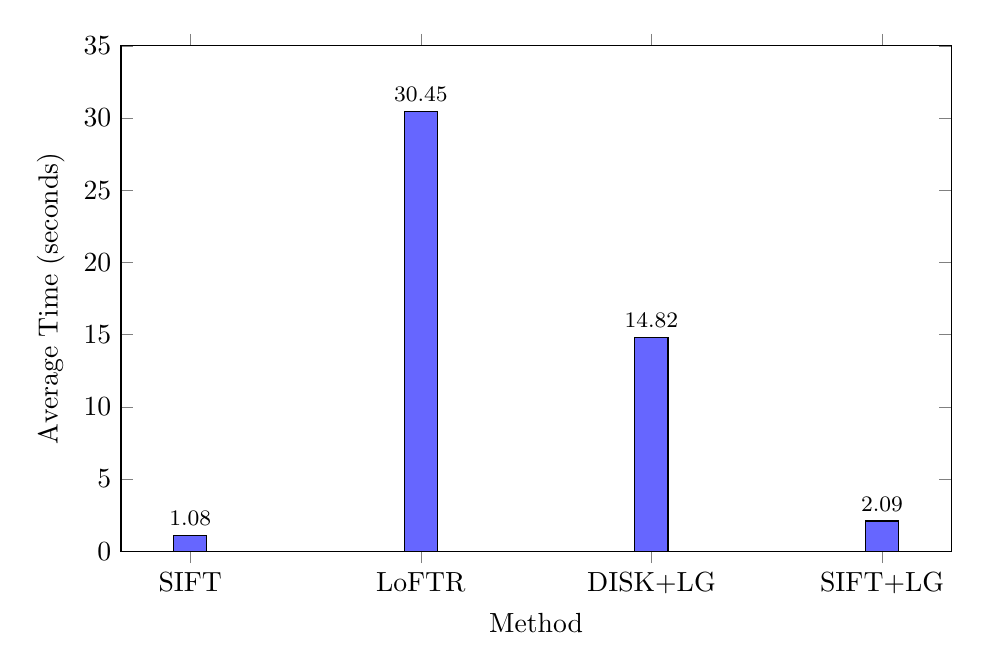
\begin{tikzpicture}
\begin{axis}[
    ybar,
    bar width=12pt,
    width=\textwidth,
    height=8cm,
    ylabel={Average Time (seconds)},
    xlabel={Method},
    symbolic x coords={SIFT, LoFTR, DISK+LG, SIFT+LG},
    xtick=data,
    ymin=0,
    ymax=35,
    legend style={at={(0.5,1.05)}, anchor=south, legend columns=1},
    nodes near coords,
    nodes near coords align={vertical},
    every node near coord/.append style={font=\footnotesize},
]
\addplot[fill=blue!60] coordinates {(SIFT, 1.08) (LoFTR, 30.45) (DISK+LG, 14.82) (SIFT+LG, 2.09)};
\end{axis}
\end{tikzpicture}
\caption{Average Execution Time Comparison (CPU)}
\label{fig:time}
\end{figure}

\begin{figure}[H]
\centering
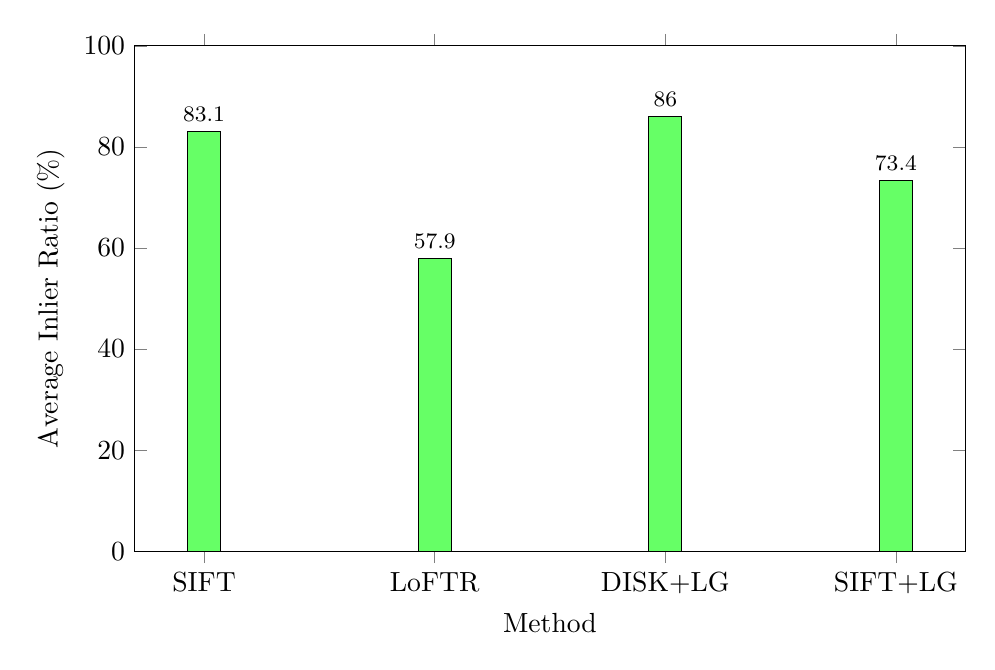
\begin{tikzpicture}
\begin{axis}[
    ybar,
    bar width=12pt,
    width=\textwidth,
    height=8cm,
    ylabel={Average Inlier Ratio (\%)},
    xlabel={Method},
    symbolic x coords={SIFT, LoFTR, DISK+LG, SIFT+LG},
    xtick=data,
    ymin=0,
    ymax=100,
    legend style={at={(0.5,1.05)}, anchor=south, legend columns=1},
    nodes near coords,
    nodes near coords align={vertical},
    every node near coord/.append style={font=\footnotesize},
]
\addplot[fill=green!60] coordinates {(SIFT, 83.1) (LoFTR, 57.9) (DISK+LG, 86.0) (SIFT+LG, 73.4)};
\end{axis}
\end{tikzpicture}
\caption{Average Inlier Ratio Comparison Across All Scenes}
\label{fig:inlier}
\end{figure}

\subsection{Visual Comparison of Match Quality}

The following figures show match visualizations for selected scenes. Green lines indicate inlier matches after RANSAC verification.

\subsubsection{Mountain Scene (Easy)}
\begin{figure}[H]
\centering
\begin{subfigure}[b]{0.48\textwidth}
    \includegraphics[width=\textwidth]{results/matches_SIFT_mountain_DSC_2839_vs_DSC_2840.jpg}
    \caption{SIFT: 1267 inliers (99\%)}
\end{subfigure}
\hfill
\begin{subfigure}[b]{0.48\textwidth}
    \includegraphics[width=\textwidth]{results/matches_LoFTR_mountain_DSC_2839_vs_DSC_2840.jpg}
    \caption{LoFTR: 4495 inliers (90\%)}
\end{subfigure}
\begin{subfigure}[b]{0.48\textwidth}
    \includegraphics[width=\textwidth]{results/matches_DISK_LightGlue_mountain_DSC_2839_vs_DSC_2840.jpg}
    \caption{DISK+LightGlue: 1174 inliers (99\%)}
\end{subfigure}
\caption{Mountain scene comparison -- All methods perform well on well-textured outdoor scenes.}
\label{fig:mountain}
\end{figure}

\subsubsection{Clock Scene (Challenging -- Repetitive Patterns)}
\begin{figure}[H]
\centering
\begin{subfigure}[b]{0.48\textwidth}
    \includegraphics[width=\textwidth]{results/matches_SIFT_clock_medium00_vs_medium01.jpg}
    \caption{SIFT: 1389 inliers (85\%)}
\end{subfigure}
\hfill
\begin{subfigure}[b]{0.48\textwidth}
    \includegraphics[width=\textwidth]{results/matches_LoFTR_clock_medium00_vs_medium01.jpg}
    \caption{LoFTR: 1541 inliers (37\%)}
\end{subfigure}
\begin{subfigure}[b]{0.48\textwidth}
    \includegraphics[width=\textwidth]{results/matches_DISK_LightGlue_clock_medium00_vs_medium01.jpg}
    \caption{DISK+LightGlue: 517 inliers (87\%)}
\end{subfigure}
\caption{Clock scene comparison -- LoFTR struggles with repetitive patterns (many false matches visible).}
\label{fig:clock}
\end{figure}

\subsubsection{Tree Scene (Challenging -- Low Texture)}
\begin{figure}[H]
\centering
\begin{subfigure}[b]{0.48\textwidth}
    \includegraphics[width=\textwidth]{results/matches_SIFT_tree_medium09_vs_medium10.jpg}
    \caption{SIFT: 301 inliers (53\%)}
\end{subfigure}
\hfill
\begin{subfigure}[b]{0.48\textwidth}
    \includegraphics[width=\textwidth]{results/matches_LoFTR_tree_medium09_vs_medium10.jpg}
    \caption{LoFTR: 664 inliers (17\%)}
\end{subfigure}
\begin{subfigure}[b]{0.48\textwidth}
    \includegraphics[width=\textwidth]{results/matches_DISK_LightGlue_tree_medium09_vs_medium10.jpg}
    \caption{DISK+LightGlue: 117 inliers (55\%)}
\end{subfigure}
\caption{Tree scene comparison -- All methods struggle with low-texture foliage. LoFTR produces many matches but most are outliers.}
\label{fig:tree}
\end{figure}

\section{Analysis and Discussion}

\subsection{Classical SIFT: Fast and Reliable Baseline}

SIFT with BruteForce matching provides an excellent baseline:
\begin{itemize}
    \item \textbf{Speed}: 30-70$\times$ faster than LoFTR on CPU
    \item \textbf{Consistency}: High inlier ratios (85-99\%) on well-textured scenes
    \item \textbf{Limitation}: Performance degrades on repetitive patterns (clock, bicycle)
\end{itemize}

\subsection{LoFTR: Dense Matching with Trade-offs}

LoFTR (Local Feature TRansformer) uses a detector-free approach with transformers:
\begin{itemize}
    \item \textbf{Strength}: Produces \textit{dense} matches (4000-7000 correspondences)
    \item \textbf{Best Case}: Achieves 99.88\% inlier ratio on dam scene
    \item \textbf{Weakness}: Struggles with repetitive structures (clock: 36.57\%, flower: 24.95\%)
    \item \textbf{Cost}: 26-33 seconds per pair on CPU (impractical without GPU)
\end{itemize}

\textbf{Key Finding}: LoFTR's dense matching produces many correspondences but can include systematic errors in repetitive regions, leading to lower inlier ratios despite accurate matches elsewhere.

\subsection{DISK+LightGlue: Best Quality-Speed Trade-off}

DISK (learned features) combined with LightGlue (learned matcher) offers:
\begin{itemize}
    \item \textbf{Quality}: Highest average inlier ratio (86\%) across all scenes
    \item \textbf{Consistency}: Maintains 80-99\% inlier ratio even on challenging scenes
    \item \textbf{Speed}: 2$\times$ faster than LoFTR
    \item \textbf{Match Count}: Moderate (500-1300 matches) -- sufficient for most applications
\end{itemize}


Using classical SIFT features with LightGlue produces surprisingly few matches:
\begin{itemize}
    \item \textbf{Observation}: Only 7-28 matches per pair (vs. 500-4000 for other methods)
    \item \textbf{Hypothesis}: LightGlue was trained on SuperPoint/DISK features; SIFT descriptors may not generalize well
    \item \textbf{Verdict}: Not recommended for production use
\end{itemize}

\section{Key Findings from Literature}

\subsection{Why Learned Matchers Outperform Classical Approaches}

Based on the LoFTR and LightGlue papers:

\begin{enumerate}
    \item \textbf{Global Context}: Transformer-based matchers consider the entire image, not just local patches
    \item \textbf{Learned Rejection}: LightGlue learns to reject outliers during matching, reducing false positives
    \item \textbf{Coarse-to-Fine}: LoFTR matches at multiple scales simultaneously
    \item \textbf{End-to-End Training}: Joint optimization of detection and matching improves consistency
\end{enumerate}

\subsection{When to Use Each Approach}

\begin{table}[H]
\centering
\caption{Recommended Use Cases}
\label{tab:recommendations}
\begin{tabular}{lp{10cm}}
\toprule
\textbf{Method} & \textbf{Best Use Case} \\
\midrule
SIFT & Real-time applications, well-textured scenes, resource-constrained environments \\
LoFTR & Offline processing where density matters, GPU available, low-texture scenes \\
DISK+LightGlue & Best for quality-critical applications, GPU recommended but works on CPU \\
\bottomrule
\end{tabular}
\end{table}

\section{Conclusion}

Our experiments reveal that:

\begin{enumerate}
    \item \textbf{Classical SIFT remains highly competitive} for well-textured scenes with 30-70$\times$ speed advantage
    \item \textbf{DISK+LightGlue provides the best quality} with consistent 80-99\% inlier ratios
    \item \textbf{LoFTR excels at dense matching} but struggles with repetitive patterns
\end{enumerate}

For panoramic stitching on CPU, the classical SIFT approach remains practical. For quality-critical applications with GPU availability, DISK+LightGlue offers the best trade-off between speed and accuracy.

\begin{thebibliography}{9}
\bibitem{sun2021loftr}
Sun, J., et al. (2021). LoFTR: Detector-Free Local Feature Matching with Transformers. CVPR.

\bibitem{lindenberger2023lightglue}
Lindenberger, P., et al. (2023). LightGlue: Local Feature Matching at Light Speed. ICCV.

\bibitem{lowe2004sift}
Lowe, D. G. (2004). Distinctive Image Features from Scale-Invariant Keypoints. IJCV.

\bibitem{tyszkiewicz2020disk}
Tyszkiewicz, M., et al. (2020). DISK: Learning Local Features with Policy Gradient. NeurIPS.
\end{thebibliography}

\end{document}
